\chapter{Experiments}

    The following chapter will explain the methodology and the results of the various experiments undertaken to validate the V2 thruster.

    \section{V1 results}


    \section{V2 experiments}
        This section presents the various experiments that were conducted with the V2 thruster, as well as improvements that were made to this thruster while operating it.
    
        \subsection{Initial LSP shots}

            \begin{figure}[!ht]
                \centering
                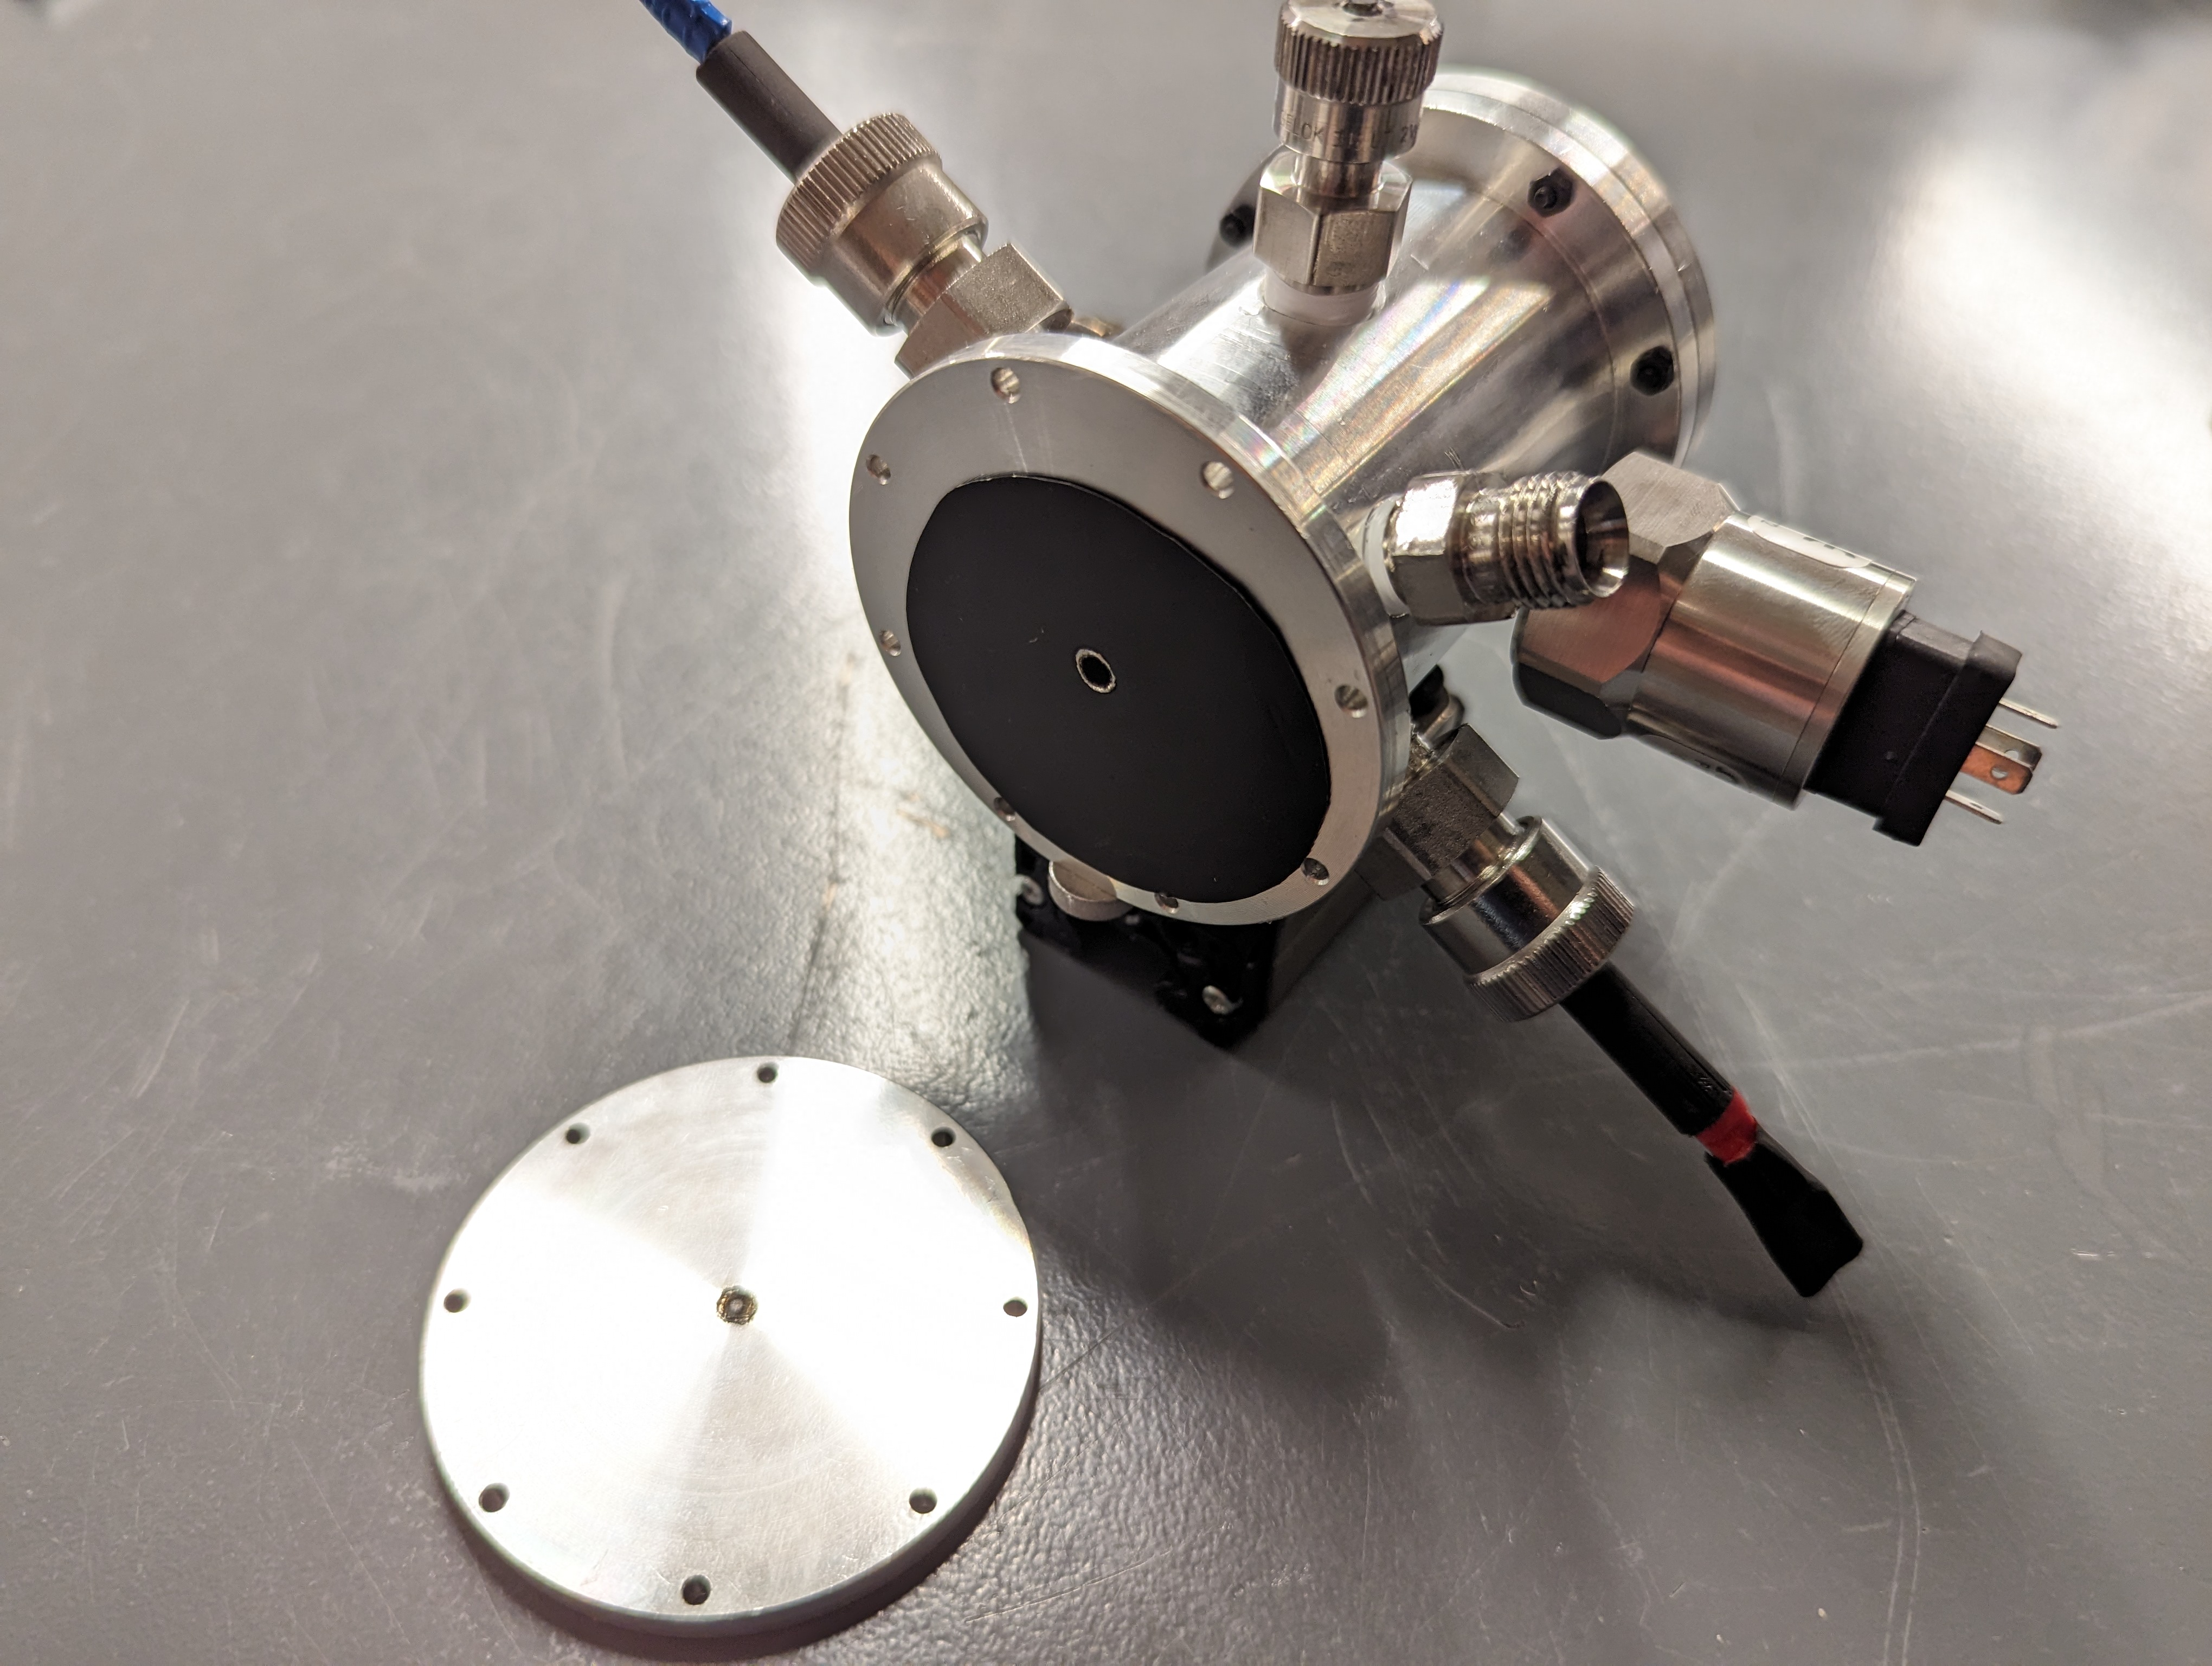
\includegraphics[width=0.75\textwidth]{assets/4 experiments/V2 test damage.jpg}
                \caption{Damage to the thruster after two \qty{3}{kW} laser shots}
            \end{figure}

            % Stills of first High-speed LSP video, showing expansion of LSP wave like in V1
        
        \subsection{Cold flow thrust tests}

            Cold flow tests were completed to give a baseline measurement of thrust before the hot fire test, and to validate the functioning of all data acquisition systems.
            
            % thrust vs pressure graph

            [FRICTION HYSTERESIS PROBLEMS] To correct these problems, a more sensitive load cell was installed with a \qtyrange{0}{5}{N} force sensing range (Honeywell FSG005WNPB). However, the issue remained.

            A different type of thrust stand (e.g. a rotating arm), could eventually be built to measure thrust in a more repeatable manner.
        
        \subsection{Effective throat area}
            
            With the cold flow thrust tests completed, the effective throat area, $A^*$, was determined. Although the throat was machined to be \qty{0.7}{mm} in diameter, boundary layer effects at this size greatly reduce the effective throat area.

            [ADD SAAD BLOWDOWN DISCUSSION]

            [CITE 2 ASME STUDIES]


        \subsection{First CW LSP}
            
            A \qty{100}{\%} power CW shot was then attempted at \qty{20}{bar} argon. 

            % photo of laser on, Spark/LSP ignition, LSP constant, laser off (LSP dying down)

            This was the first CW LSP generated in the lab. No damage was noticed to the apparatus after this test.

        \subsection{Window extension tube}
            
            After the first CW LSP, more CW and pulsed shots were attempted. These continued to damage the rear window. Eventually, a \qty{3}{s} CW shot melted it severely enough that 

            \begin{figure}[!ht]
                \centering
                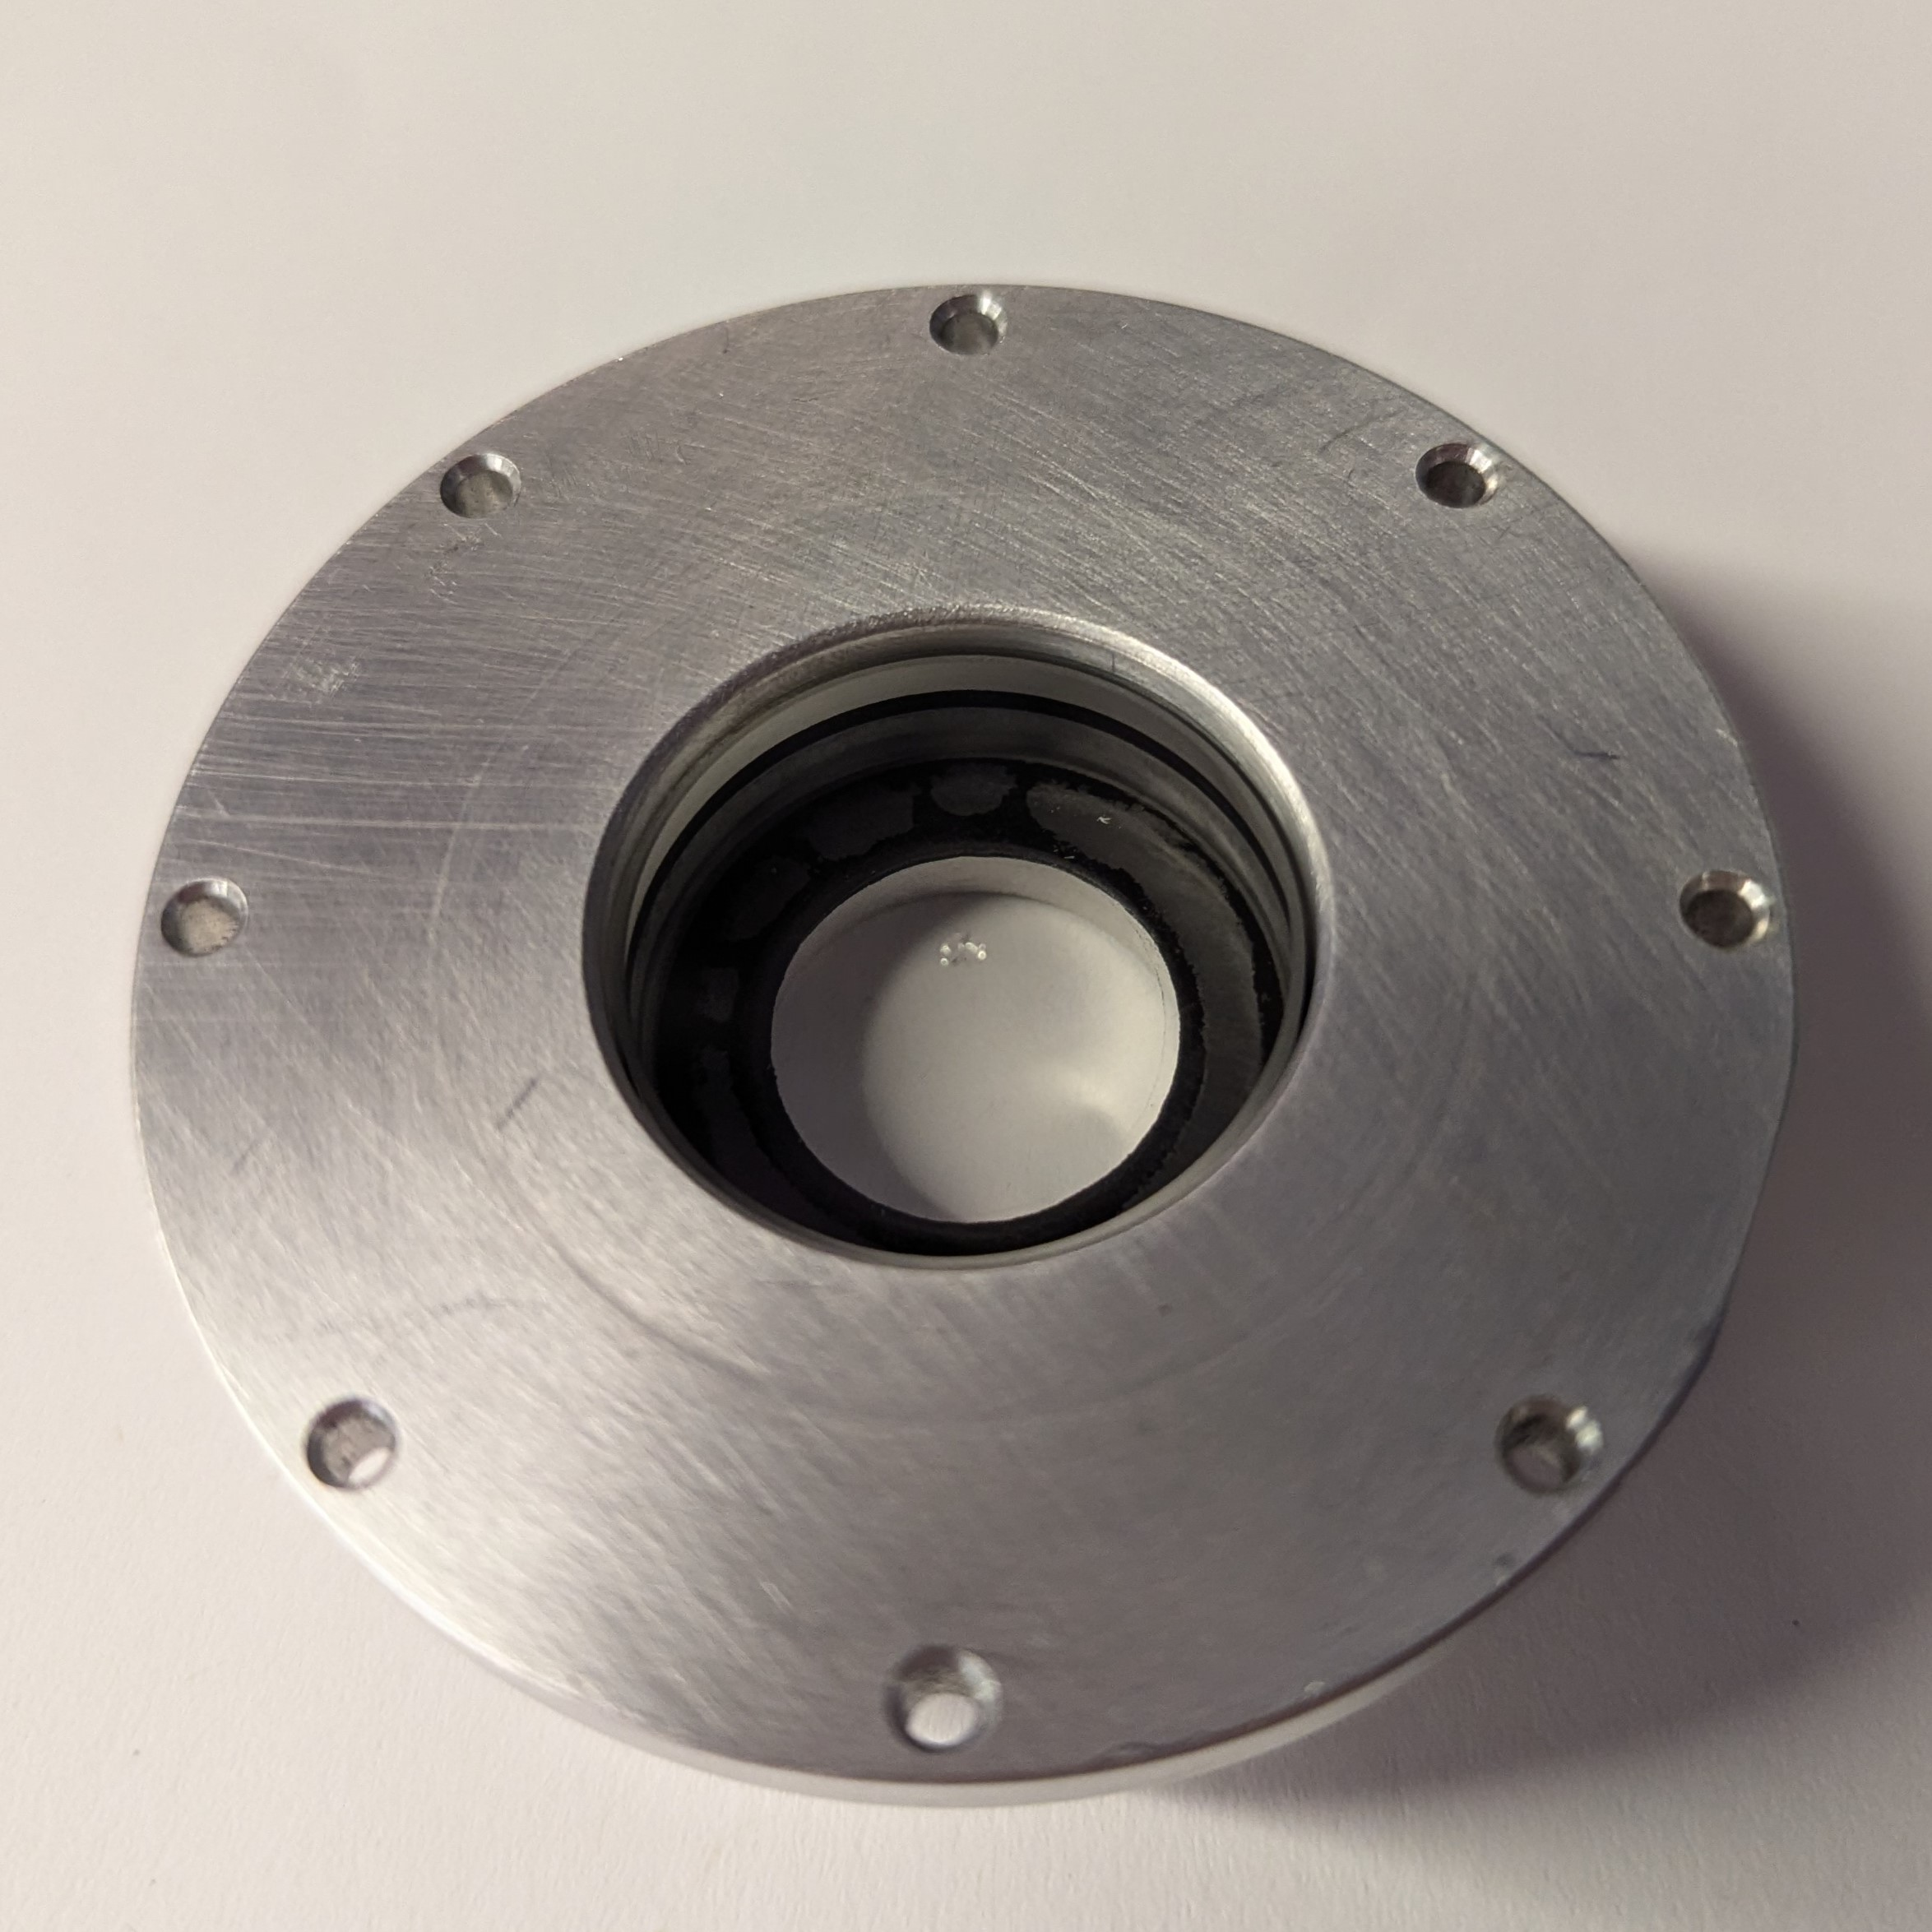
\includegraphics[width=0.5\textwidth]{assets/4 experiments/window damage.jpg}
                \caption{Rear window damage on V2}
            \end{figure}

            The solution chosen was to manufacture a window extension tube, moving the rear window downstream to where the laser flux density is comparable to the front window, where no damage was seen.

            [drawing of extension tube]


        


        % \subsection{CW LSP (hot fire) thrust tests}

        %     Find m dot, show thrust graph. Get Isp from these. Compare to other thrusters in the literature. Get heat deposition efficiency somehow? Or use Toyoda's definition of efficiency that only uses power in.

        \section{Summary of results}

            \begin{table}[]
                \caption{Summary of the studied V2 thruster characteristics}
                \label{tab:characteristics}
                \begin{tabular}{ll}
                Characteristic             & Value and unit \\
                mdot                       &                \\
                Valve A*                   &                \\
                Nozzle A*                  &                \\
                Internal volume            &                \\
                Cold flow thrust at 20 bar &               
                \end{tabular}
            \end{table}
 

            

        



